\subsection{实验目的}
理解遥感信号处理的概念,学习雷达信号处理中的线性调频信号及其脉冲压缩技术。通过实验了解线性调频信号的性质,并实现线性调频信号的脉冲压缩。
\subsection{实验原理}
\subsubsection{离散时间信号的线性卷积}

\begin{equation}
\begin{split}
y(n) =& s(n) \otimes h(n) \\
=& \sum_{m=0}^{M-1} s(n - m)h(m) \\
=& \sum_{m=n-(M-1)}^{n} s(m)h(n - m) \\
\end{split}
\end{equation}
\subsubsection{傅立叶变换的性质}
\begin{eqnarray}
g_1(t)\otimes g_2(t) &\leftrightarrow& G_1(f)G_2(f) \\
g_1(t)g_2(t) &\leftrightarrow& G_1(f)\otimes G_2(f) \\
\end{eqnarray}
\begin{eqnarray}
g(t - t_0) &\leftrightarrow& G(f)\exp(-\jj 2\pi ft_0) \\
g(t)\exp(\jj 2\pi f_0t) &\leftrightarrow& G(f-f_0)
\end{eqnarray}
\subsubsection{补零}
在离散时间下,某一域中的序列补零相当于对另一域进行升采样。这使得另一域中的数据量增大,但是不会改变序列的信息内容。
\subsubsection{线性调频信号}
\begin{equation}
s(t) = \rect\left( \frac{t}{T} \right)\exp(\jj\pi\gamma t^2)
\end{equation}
其中
\begin{description}
	\item[t] 时间变量,单位为秒。
	\item[T] 脉冲持续时间。
	\item[$\gamma$] 线性调频率,单位为Hz/s。
\end{description}
\begin{equation}
\rect(x) = \begin{cases}
1, \quad \abs{x} \leq 0.5 \\
0, \quad\text{其他}
\end{cases}
\end{equation}
\begin{description}
	\item[相位$\phi$] $\phi(t) = \pi\gamma t^2$
	\item[频率] $f=\frac{1}{2\pi}\frac{\dd\phi(t)}{\dd t}$
	\item[带宽] $BW=\abs{\gamma}t$
	\item[时宽带宽积] $TBP=\abs{\gamma}T^2$
\end{description}
线性调频信号的频谱函数
\begin{equation}
S(f)=\rect\left(\frac{f}{\gamma T}\right)\exp\left( -\jj\pi\frac{f^2}{\gamma} \right)
\end{equation}
\subsubsection{线性调频信号的采样}
基带复线性调频信号的最大频率为$\frac{\abs{K}T}{2}$,所以最低复采样率$f_s$必须大于带宽$\abs{K}T$,定义过采样因子
\begin{equation}
\alpha=\frac{f}{\abs{K}T}
\end{equation}
应选在$1.1-1.4$之间。
\subsubsection{脉冲压缩}
在探测系统中,通过脉冲能量可以对远场目标的距离、速度、反射率等进行测量。为了使得测量有效,接收脉冲必须具有足够的能量和足够好的分辨率。如果发射脉冲的持续时间为$T$,则每一个目标在回波数据中占有相同的时间间隔$T$,故压缩前的可分辨能力为
\begin{equation}
\rho = T
\end{equation}
在任意时刻,回波中间隔大于这一时间的两个目标都不会被同一个脉冲同时照射到。因此,为了得到更好的分辨率,必须使用短脉冲或经过信号处理能得到短脉冲的信号。
\paragraph{频域中脉冲压缩的本质}
将信号频谱域含有二次共轭相位的频域滤波器进行相乘。也称为匹配滤波。
\begin{eqnarray}
s_{out}(t) &=& s_r(t)\otimes h(t) \\
s_{out}(t) &\approx& T\mathrm{sinc}(\gamma T( t-t_0 )) \\
h(t) &=& g^*(-t)
\end{eqnarray}
其中,发射信号
\begin{equation}
s(t) = \rect\left(\frac{t}{T}\right)\exp\left( \jj\pi\gamma t^2 \right)
\end{equation}
$t_0$延时后的目标回波
\begin{equation}
s_r(t) = \rect\left(\frac{t-t_0}{T}\right)\exp\left(\jj\pi\gamma(t-t_0)^2\right)
\end{equation}
滤波器冲击响应函数
\begin{equation}
h(t) = \rect\left(\frac{t}{T}\right)\exp(-\jj\pi\gamma(-t)^2) = \rect\left(\frac{t}{T}\right)\exp(-\jj\pi\gamma t^2)
\end{equation}
\paragraph{频域匹配滤波器}
发射信号
\begin{eqnarray}
s(t) &=& \rect\left(\frac{t}{T}\right)\exp(\jj\pi\gamma t^2) \\
S(f) &=& \rect\left(\frac{f}{\abs{\gamma}T}\right)\exp\left(-\jj\pi\frac{f^2}{\gamma}\right)
\end{eqnarray}
回波信号
\begin{eqnarray}
s_r(t) &=& \rect\left(\frac{t-t_0}{T}\right)\exp(\jj\pi\gamma(t - t_0)^2) \\
S_r(f) &=& \rect\left(\frac{f}{\abs{\gamma}T}\exp\left(-\jj\pi\frac{f^2}{\gamma}\right)\right)\exp(-\jj2\pi t_0f) \\
\end{eqnarray}
匹配滤波器系统函数
\begin{eqnarray}
H(f) &=& \rect\left(\frac{f}{\abs{\gamma}T}\right)\exp\left(\jj\pi\frac{f^2}{\gamma}\right)
\end{eqnarray}
输出信号
\begin{eqnarray}
S_{out}(f) &=& S_r(f)H(f) = \rect\left(\frac{f}{\abs{\gamma}T}\right)\exp(-\jj2\pi ft_0) \\
s_{out}(t )&=& \abs{\gamma}T\sinc(\gamma T(t-t_0))
\end{eqnarray}
\paragraph{频域匹配滤波器的三种生成方式}
\begin{enumerate}
	\item 将时间翻折后的复制脉冲取复共轭,计算补零DFT。
	\item 复制脉冲补零后进行DFT,对结果取复共轭。
	\item 根据设定的线性调频率特性,直接在频域生成匹配滤波器。
\end{enumerate}
\subsection{实验流程}
\begin{figure}[H]
	\centering
	\includegraphics[width=0.6\linewidth]{figure/PulseCompression1Flowchart.pdf}
	\caption{脉冲压缩流程图}
\end{figure}
\subsection{实验程序}
\lstinputlisting[caption={脉冲压缩程序}]{"../Executable Script/Exp 11/PulseCompression.m"}
\subsection{实验结果和分析}
生成100MHz带宽的线性调频信号,对其进行频谱分析,可以得到如下图所示的频谱图。
\begin{figure}[H]
	\centering
	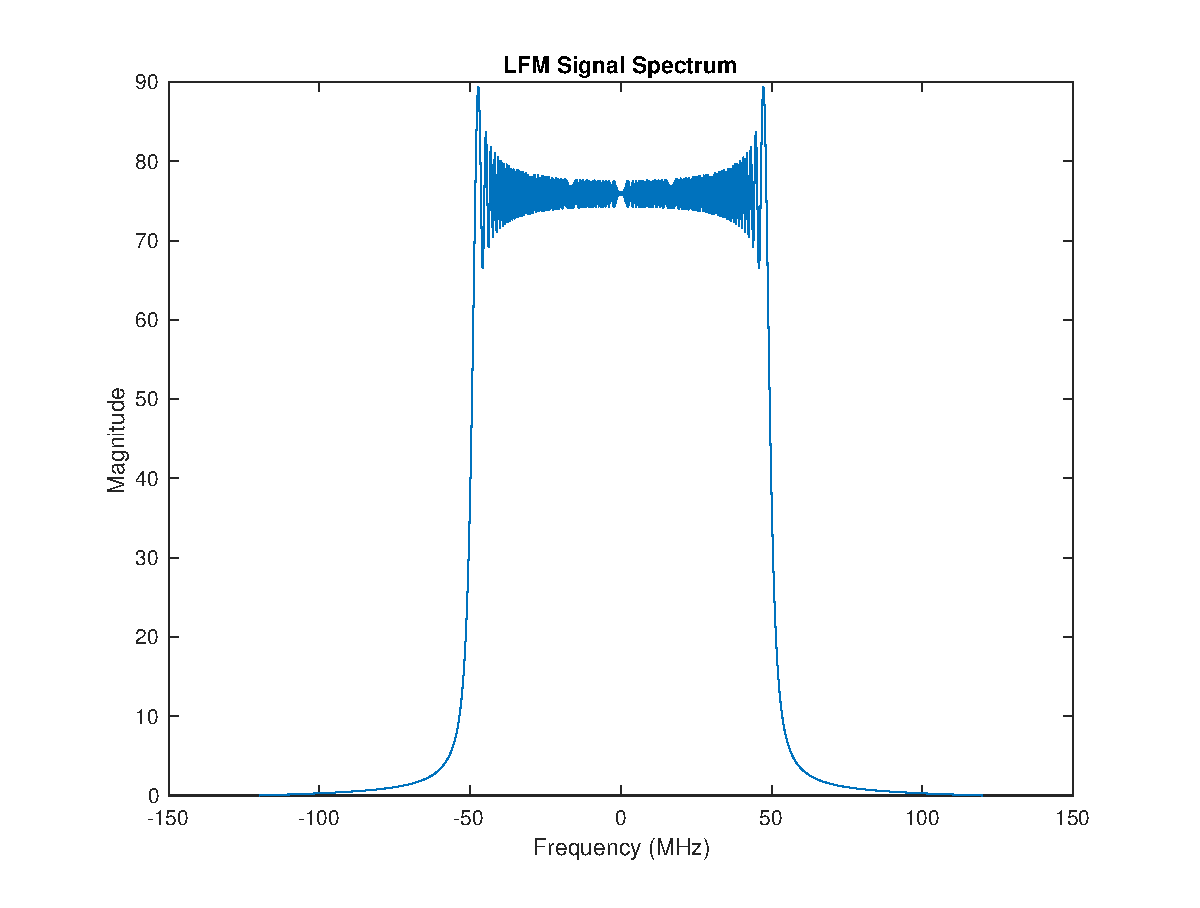
\includegraphics[width=0.7\linewidth]{figure/LFMSignalSpectrum.eps}
	\caption{线性调频信号频谱}
\end{figure}
对线性调频信号参考信号延迟17$\mu$s,生成模拟回波信号
\begin{figure}[H]
	\centering
	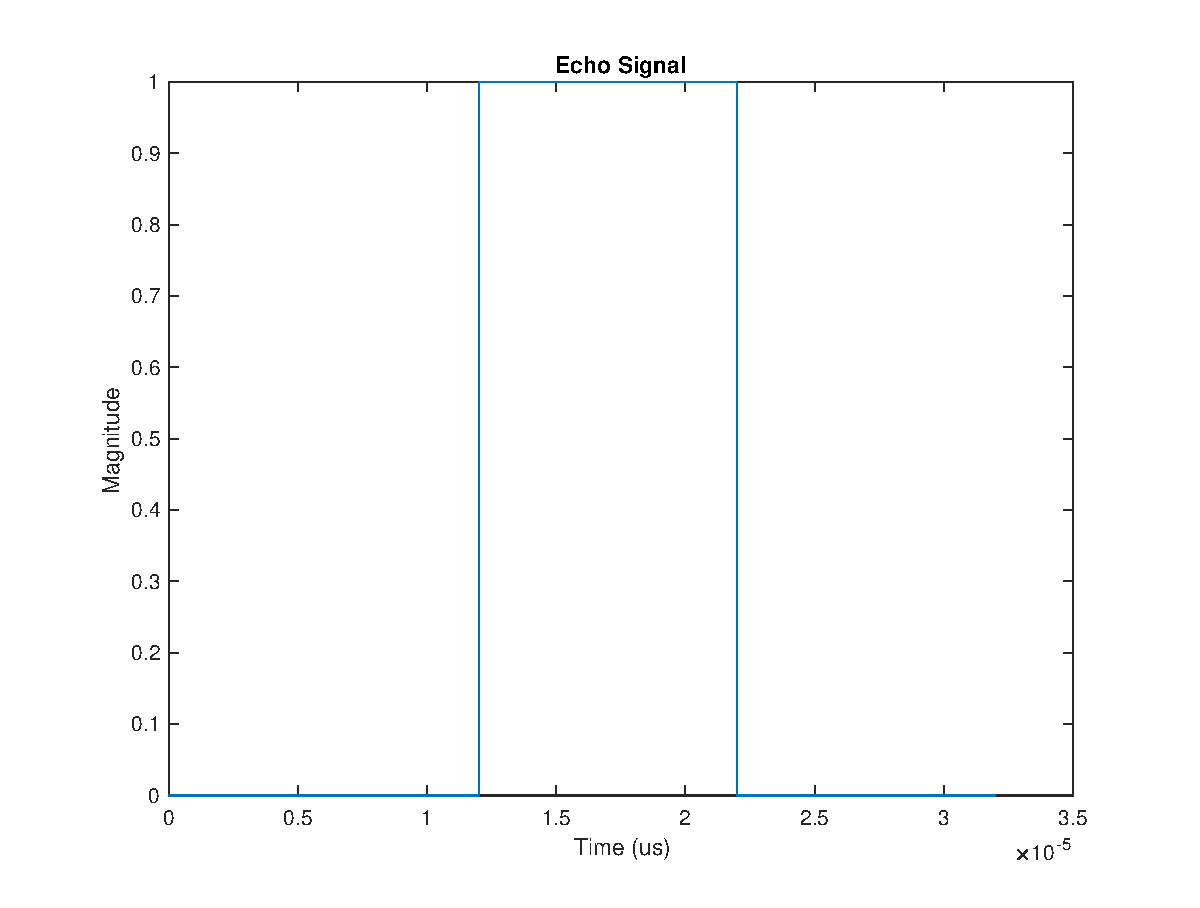
\includegraphics[width=0.7\linewidth]{figure/LFMEchoSignal.eps}
	\caption{模拟回波信号}
\end{figure}
对回波信号分别进行通过不同方式生成匹配滤波器的脉冲压缩。通过时域线性卷积可以得到脉冲压缩的结果如下图所示。
\begin{figure}[H]
	\centering
	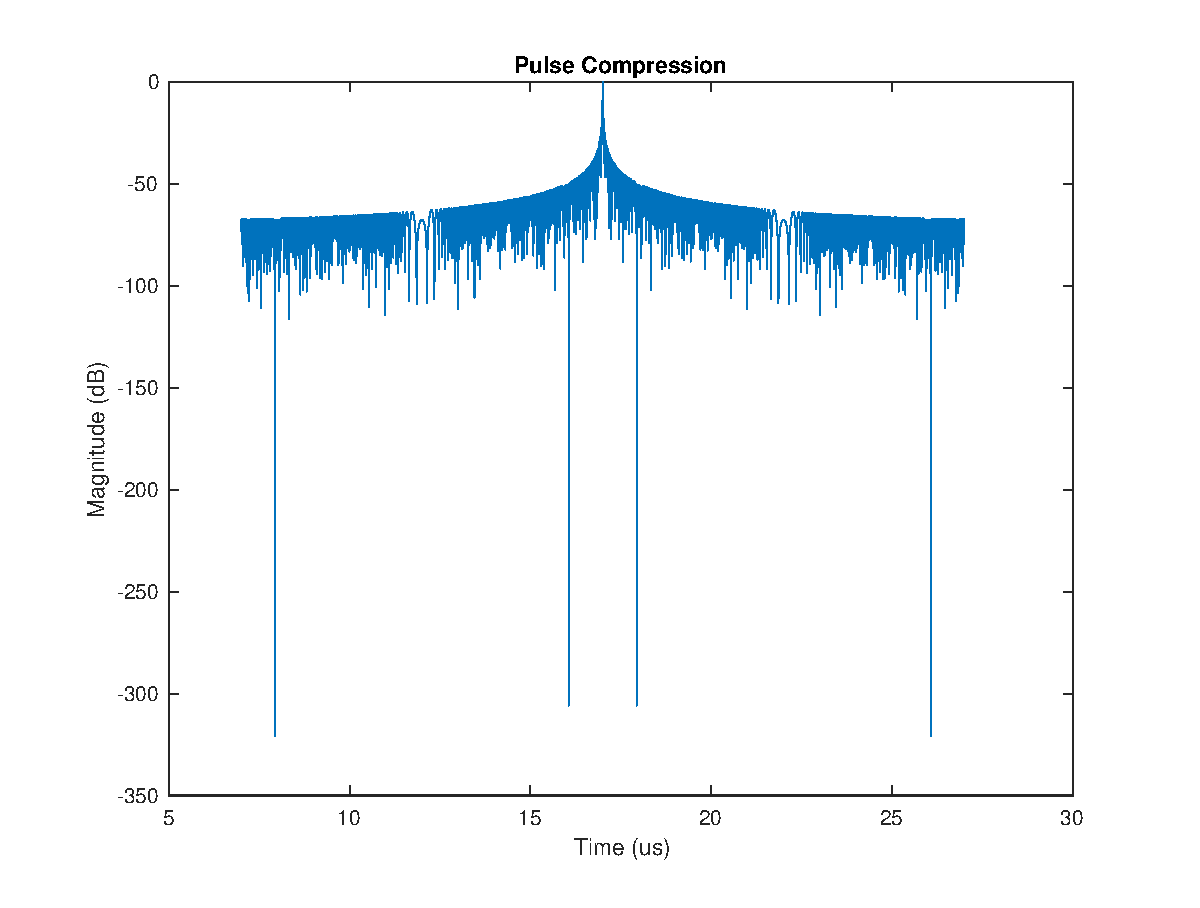
\includegraphics[width=0.7\linewidth]{figure/LinearConvolutionPulseCompression.eps}
	\caption{通过时域线性卷积实现的脉冲压缩}
\end{figure}
通过对参考信号傅立叶变换后共轭得到对匹配滤波器的频域脉冲压缩结果如下图所示。
\begin{figure}[H]
	\centering
	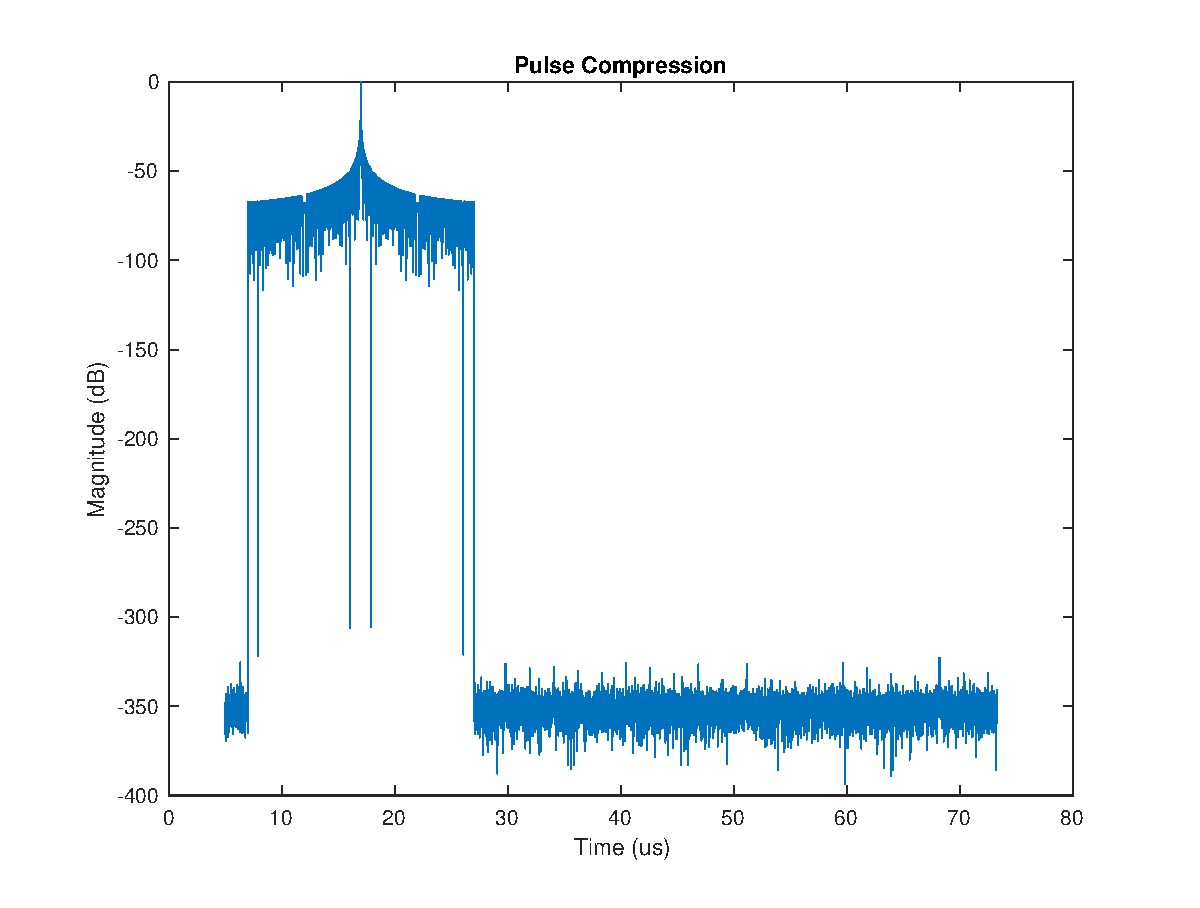
\includegraphics[width=0.7\linewidth]{figure/FFTConjuagePulseCompression.eps}
	\caption{参考信号傅立叶变换后共轭得到的匹配滤波器脉冲压缩}
\end{figure}
通过对参考信号翻转共轭傅立叶变换后得到对匹配滤波器的脉冲压缩结果如下图所示。
\begin{figure}[H]
	\centering
	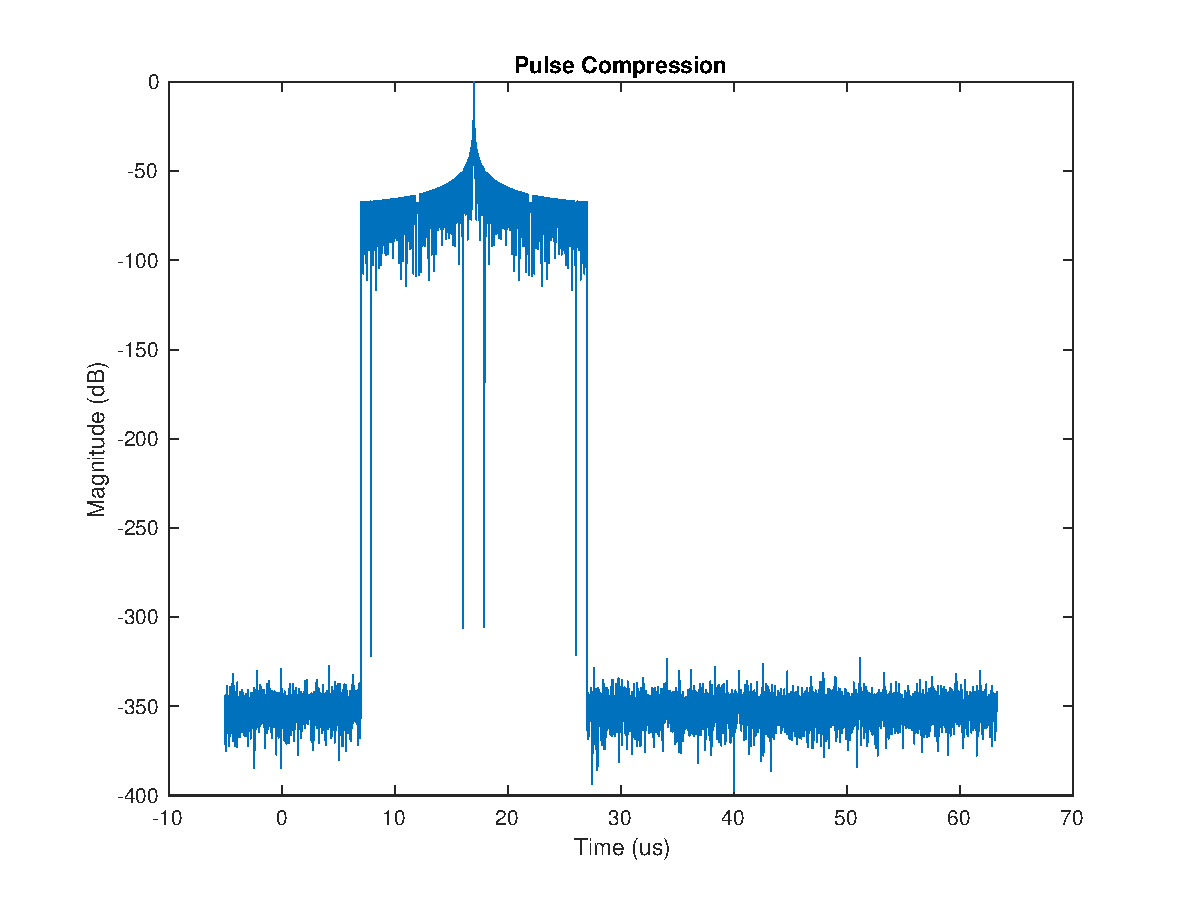
\includegraphics[width=0.7\linewidth]{figure/FilpConjugateFFTPulseCompression.eps}
	\caption{参考信号翻转共轭傅立叶变换得到的匹配滤波器脉冲压缩}
\end{figure}
可以看到,使用四种方法都可以得到脉冲压缩的结果。由于参考信号是一个关于0的共轭反对称信号,所以在进行脉冲压缩后,$\sinc$函数峰值所在的位置不尽相同,这是由于离散傅立叶变换的性质决定的,所以根据傅立叶变换的性质对脉冲压缩对结果进行相应的横坐标的设定,就可以得到正确的结果。